




\chapter[基于二维滑动窗口的图像分类神经网络显著图增强方法]{\texorpdfstring{基于二维滑动窗口的图像分类神经网络\\显著图增强方法}{基于二维滑动窗口的图像分类神经网络显著图增强方法}}

\thispagestyle{others}
\pagestyle{others}
\xiaosi




\section{问题描述和研究思路}

显著图分辨率低,包含特征细节信息少仍然是当前绝大多数显著图解释方法的一个弊病。从基于卷积神经网络的图像分类神经网络来看,针对这一网络的显著图解释方法通常是从卷积神经网络的最后一层卷积层提取特征图。这一层包含了丰富的类别特征信息,然后通过加权组合这些特征图来生成最终的显著图。然而,由于卷积神经网络的结构特性,最后一层卷积层会输出多个通道的低分辨率特征图。因此,无论怎样组合这些特征图,最终得到的显著图分辨率仅与最后一层卷积层的单一通道特征图相当。当然,为了建立显著图与原始输入图片的特征对应关系,通常会对原始输入图片进行分辨率放大。这一过程通常采用双线性插值算法,但这并不意味着显著图中有效信息的增加。另外,当前的一些研究者也在积极探索对基于Tansformer架构的图像分类模型进行显著图解释,H. Chefer等人\textsuperscript{\cite{chefer2021transformer}}在近年发布了针对这一方面的研究,他们针对Transformer的结构的制定了新的层间相关性反向传播规则,解决了传播过程中遇到的注意层和跳跃连接时的挑战。他们将每一个Transformer块的梯度和其对应的相关性分数结合解决了Transformer在图像分类领域的显著图可视化问题。但是即便如此他们针对Transformer提出的方法仍然会面临低分辨率的困扰,究其原因是Transformer结构的图像分类神经网络反向传播过程中计算并生成显著图时也只能受限于token的尺寸,无法生成包含信息量更多的显著图。图\ref{fig:motivation}描述了这一问题,无论针对卷积神经网络的基于类激活映射图的方法还是针对Transformer架构提出的Transformer attribution方法(即Chefer等人提出的方法)都只能生成分辨率较低的原始显著图,之后通过上采样获得最终的显著图。

\begin{figure}[h]
	\centering 
	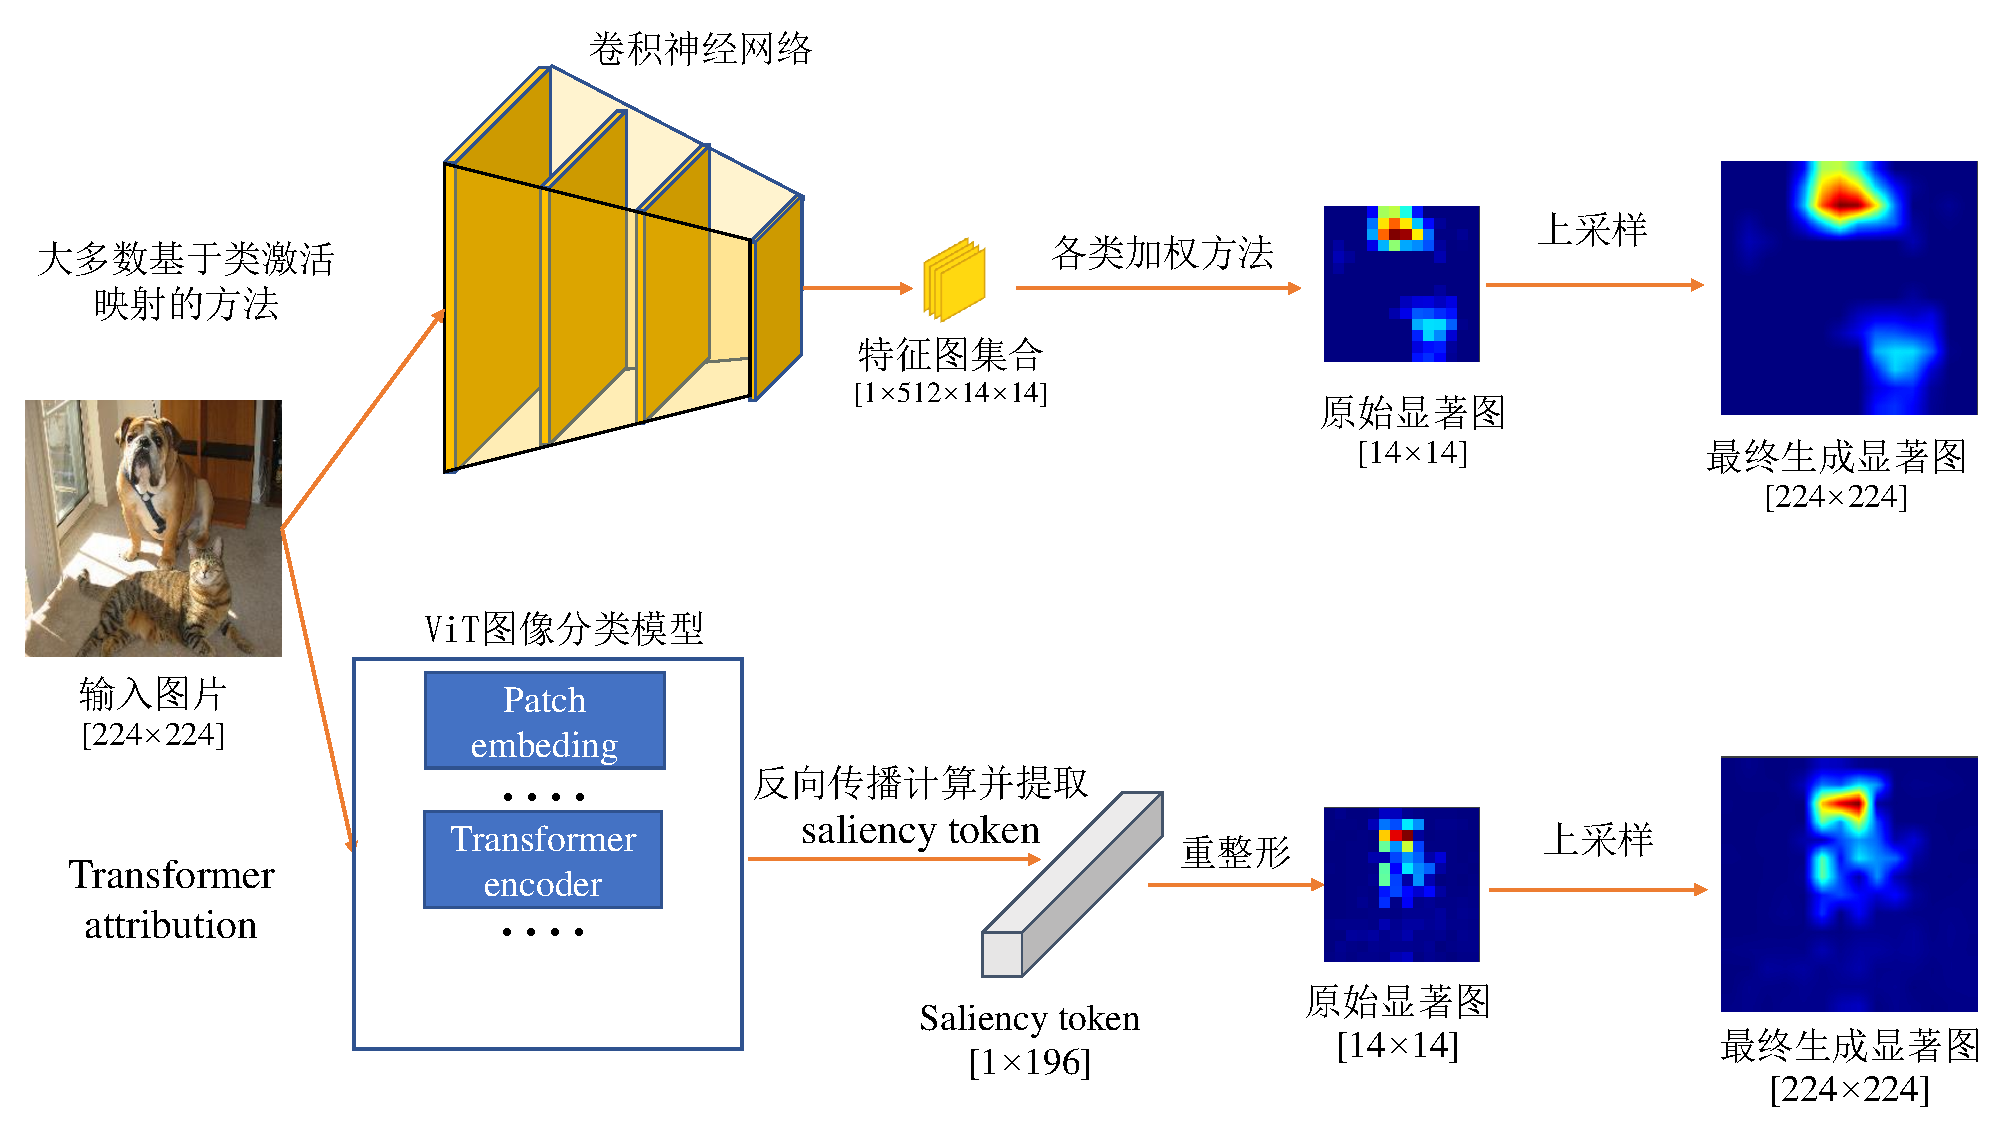
\includegraphics[width=15cm]{fig/ch4/motivation.pdf}
	\bicaption[\xiaosi 当前显著图解释方法分辨低的原因]{\wuhao 当前显著图解释方法分辨低的原因}{\wuhao Reasons for the low resolution of current saliency map interpretation methods}
	\label{fig:motivation}
\end{figure}


因此为了解决上述的问题,本章提出了一种通用的显著图增强方法,可以直接应用在多数可视化算法上。该方法使用固定尺寸的滑动窗口对输入图片中的所有局部区域上采样到输入图片尺寸,然后将结果输入到选定的可视化算法中得到所有图片的针对特定类别的显著图和概率分数,最后将显著图下采样到输入图片对应位置上的窗口中,并乘以概率分数,即可得到具备更多细节的显著图。将该方法应用在不同的可视化算法上,这些算法基于不同架构的网络,无论是量化指标还是直观评测都显示出本章的方法使这些可视化算法得到了明显提升,从而证明本章提出的方法的有效性和可靠性。


\section{基于二维滑动窗口的图像分类神经网络显著图增强方法}
为了解决当前可视化算法存在的分辨率低,特征模糊,噪声多的问题,本章提出的方法在输入图片上应用了滑动窗口,通过采集并融合不同窗口图片的可视化信息,让可视化算法加强对输入图片中的局部信息的感知。具体的算法流程图展示在图\ref{fig:pipeline}中。

\begin{figure}[h]
	\centering 
	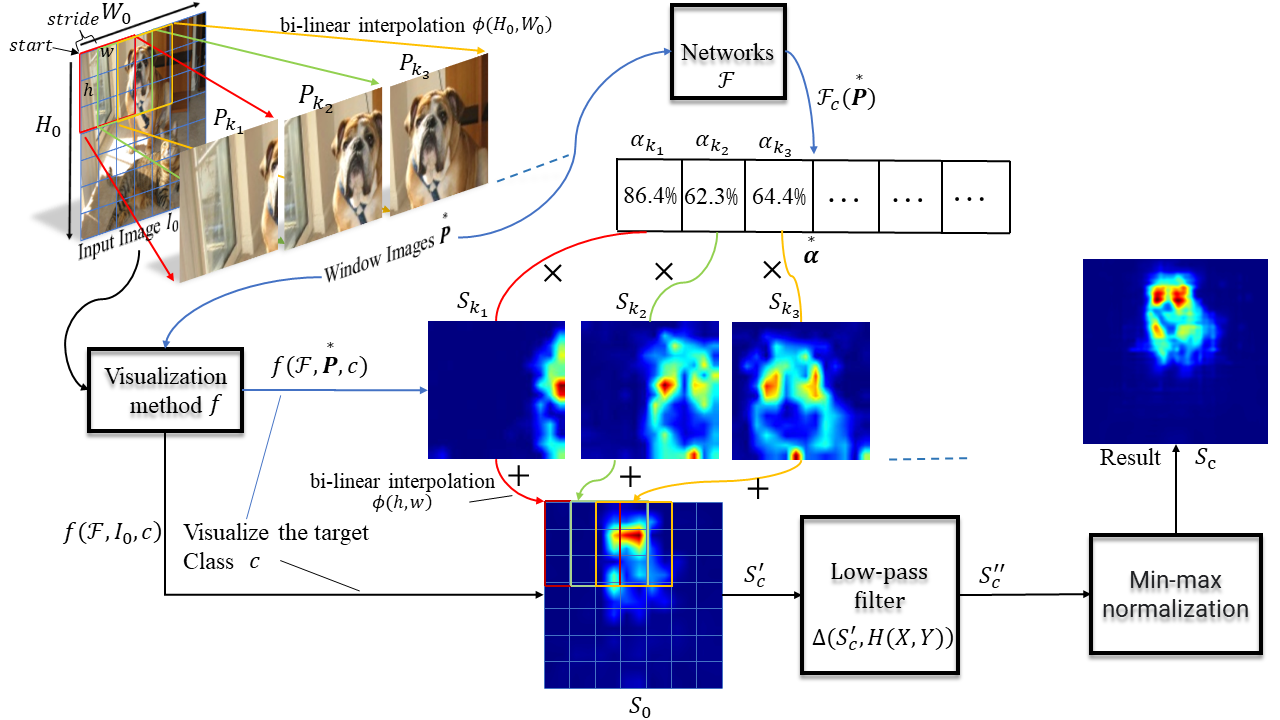
\includegraphics[width=15cm]{fig/ch4/pipeline.png}
	\bicaption[\xiaosi 显著图增强方法的流程图]{\wuhao 显著图增强方法的流程图}{\wuhao Pipeline of the saliency map enhancement approach}
	%	\bicaption[\xiaosi MSG-CAM算法流程示意图]{\wuhao MSG-CAM算法流程示意图}{\wuhao Pipeline of MSG-CAM}
	\label{fig:pipeline}
\end{figure}

\subsection{获取窗口图片集合}
设定原始输入图片$I_0 \in \mathbb{R}^{3\times H_0 \times W_0}$,使用一个二维滑动窗口函数$\psi$来从输入图片$I_0$中提取窗口图片,函数$\psi(I, start, h, w, stride)$中$I$就是函数所应用的输入图片,$start$表示滑动窗口在二维坐标系统的起点,一般设定在输入图片的左上角位置,$h$和$w$表示窗口像素尺寸且窗口尺寸应该小于输入图片尺寸,$stride$表示每次滑动窗口移动的像素个数,窗口从左上角起点开始移动,只能在图片区域内移动,即滑动窗口应该向右或者向左移动。每次移动则将窗口内的图片区域进行复制并保存,移动完毕后即可得到关于窗口图片的集合,单张窗口图片的获取的公式如下:
\begin{equation}
	p_{k_n}=\psi(I_0,start,h,w,stride)
	\label{pkn}
\end{equation}
式\ref{pkn}中$p_{k_n}$表示一张窗口图片,$k_n$表示这张图片在输入图片$I_0$中的二维坐标标记。所有窗口图片的集合可以如下表示:
\begin{equation}
	\overset{*}{\bm{p}}=\{p_{k_1},p_{k_2},\cdots,p_{k_n}\}
\label{ps}
\end{equation}
式\ref{ps}中,$\overset{*}{\bm{p}}$即表示滑动窗口所有窗口图片集合。获取的窗口图片尺寸是和窗口一致的,因此是无法直接输入图像分类模型的,所以需要将其上采样到原始输入图片$I_0$的尺寸,本方法上采样所用的函数是双线性插值函数$\phi$,具体上采样过程描述见如下公式:
\begin{equation}
	\overset{*}{\bm{P}}=\phi(\overset{*}{\bm{p}},H_0,W_0) 
\label{Ps}
\end{equation}
式\ref{Ps}中,$H_0$和$W_0$是原始输入图片$I_0$的长和宽的像素个数,$\overset{*}{\bm{P}}$表示窗口图片上采样后的图片集合,因此 $\overset{*}{\bm{P}}=\{P_{k_1},P_{k_2},\cdots,P_{k_n}\}$,$P_{k_n}$即表示窗口图片$p_{k_n}$上采样到原始输入图片尺寸后的图片。

\subsection{获取窗口图片的显著图和权重}
设定$\mathcal{F}$是经过预训练的图像分类神经网络,$\mathcal{F}_c(I)$表示当输入图片是$I$的情况下,图像分类神经网络$\mathcal{F}$关于类别$c$的输出概率分数。对于当前主流的显著图解释算法来说,将某一显著图解释算法考虑为一个函数$f$,该函数的输入参数是图像分类神经网络$\mathcal{F}$,输入图片$I$和指定类别$c$。当输入图片是$I_0$,可以获得图像分类神经网络$\mathcal{F}$在采用显著图解释算法$f$时生成的关于类别$c$的显著图:
\begin{equation}
	S_0=f(\mathcal{F},I_0,c)
	\label{S0}
\end{equation}
式\ref{S0}是生成的显著图,且$S_0 \in \mathbb{R}^{1\times H_0 \times W_0}$。显著图$S_0$的分辨率和原始输入图片是一致的,因其已经经过上采样处理了。$S_0$中的像素和原始输入图片的像素是一一对应的,且其像素的值表示图像分类神经网络对输入图片$I_0$关于类别$c$的判断权值。现在已经获得了原始输入图片$I_0$的显著图,在上一小节当中,获取的窗口图片集合$\overset{*}{\bm{P}}$也需要经过同样的步骤分别获取每张窗口图片关于类别$c$的显著图:
\begin{eqnarray}
	\overset{*}{\bm{S}} &=& f(\mathcal {F}, \overset{*}{\bm{P}},c) \nonumber \\
	~ &=& \{S_{k_1},S_{k_2},\cdots,S_{k_n}\}
	\label{eq:Ss}
\end{eqnarray}
式\ref{eq:Ss}中$\overset{*}{\bm{S}}$表示图像分类神经网络$\mathcal{F}$对窗口图片集合生成的关于类别$c$的显著图集合,$\overset{*}{\bm{S}}$中所有显著图的分辨率都和原始输入图片$I_0$一致。

在所有基于类激活映射的显著图解释算法中,都采用了各种形式的特征图加权,而这一步骤对于衡量每个特征图关于类别$c$的贡献至关重要。为了衡量由不同窗口图片生成的显著图的重要性,可以获得每张窗口图片相对于类别$c$的概率分数。这个概率分数反映了图像分类神经网络关于窗口图片中类别$c$的特征信息的贡献权重。
\begin{eqnarray}
	\overset{*}{\bm{\alpha}} &=& \mathcal{F}_c(\overset{*}{\bm{P}}) \nonumber \\
	~ &=& \{\alpha_{k_1},\alpha_{k_2},\cdots,\alpha_{k_n}\}
\label{eq:alpha}
\end{eqnarray}
式\ref{eq:alpha}中$\overset{*}{\bm{\alpha}}$就是$\overset{*}{\bm{P}}$所有窗口图片的关于类别$c$的概率分数,以此作为$\overset{*}{\bm{S}}$的权重。

\subsection{融合窗口图片集合的显著图}
由于不同窗口图片生成的显著图只包含了原始输入图片部分区域的特征信息,因此需要将所有窗口图片进行拼接融合从而得到包含丰富特征信息的完整显著图,这一将窗口图片显著图拼接融合的操作也变相提高了最终呈现特征图对细节特征的解释能力,能够给出更精确的特征信息。由于式\ref{eq:ss}中窗口图片显著图集合$\overset{*}{\bm{S}}$中的显著图尺寸和原始输入图片$I_0$的分辨率是一致的,因此要将其下采样至窗口图片的尺寸才方便根据其携带的在原始输入图片中的坐标信息进行拼接融合,具体的过程用公式表示如下:
\begin{eqnarray}
	\overset{*}{\bm{s}} &=& \phi(\overset{*}{\bm{S}},h,w) \nonumber \\
	~ &=& \{s_{k_1},s_{k_2},\cdots,s_{k_n}\}
\label{eq:ss}
\end{eqnarray}
式\ref{eq:ss}中,$\overset{*}{\bm{s}}$是窗口图片集合$\overset{*}{\bm{P}}$的显著图集合$\overset{*}{\bm{S}}$下采样至滑动窗口尺寸的显著图集合,$s_{k_n}$中的$k_n$表示该张显著图在原始输入图片中的坐标位置,这个坐标位置是用来方便后续显著图进行拼接融合的。

显著图拼接融合的具体方法是将所有$\overset{*}{\bm{s}}$中窗口尺寸的显著图乘以该显著图在$\overset{*}{\bm{\alpha}}$对应的权重,再根据记录的坐标和原始输入图片的显著图$S_0$中对应位置区域的像素值相加,窗口显著图拼接融合的具体公式如下:
\begin{eqnarray}
	S^{\prime}_c &=& \sum(\overset{*}{\bm{s}}\overset{*}{\bm{\alpha}}+S_0) \nonumber \\
	~ &=& \sum_{k_1}^{k_n}(\alpha_{k_n}s_{k_n}+S_0^{k_n})
	\label{eq:s'}
\end{eqnarray}
在式\ref{eq:s'}中,$S_0^{k_n}$中$k_n$表示原始输入图片的显著图$S_0$中左上角坐标为$k_n$长宽为$h$和$w$的窗口区域。$S^{\prime}_c$表示拼接融合后的显著图。

\subsection{平滑和归一化显著图}
因为滑动窗口是以一定步长在输入图片上截取窗口图片,这会导致窗口图片的显著图的在按照以上方法进行融合的过程中不可避免的会在拼接融合后的显著图上留下网格状的痕迹,使得显著图视觉效果不够平滑。因此为了尽可能降低滑动窗口带来的不利影响,本方法使用了一个理想低通滤波器对其进行优化,将显著图中网格状的痕迹进行减弱或者消除。定义这个理想低通滤波器函数为$\delta$,$S^{\prime}_c$经过其处理的过程由以下式子定义:

\begin{equation}
	S^{\prime\prime}_c= \Delta(S_c^{\prime},H(X,Y))
	\label{eq:s''}
\end{equation}
式\ref{eq:s''}中,$H(X,Y)$为该理想低通滤波器的传递函数,它的具体定义如下:
\begin{equation}
	H(X,Y)=\left\{
	\begin{aligned}
		1 &&& D(X,Y)\leq D_0 \\
		0 &&& D(X,Y) > D_0
	\end{aligned}
	\right.
	\label{eq:hxy}
\end{equation}
在式\ref{eq:hxy}中,$D_0$是截止频率到频率域中心的距离,它决定了低通滤波器的频率响应范围。当$D(X,Y)$小于$D_0$时,$H(X,Y)$接近于1,表示对低频分量的保留;当$D(X,Y)$大于等于$D_0$时,$H(X,Y)$接近于0,表示对高频分量的抑制。因此,$D_0$决定了滤波器的频率截止位置,即在该位置之前的频率成分会被保留,之后的频率成分会被抑制。$D(X,Y)=\sqrt{X^2+Y^2}$是显著图$S^{\prime}_c$的频率域里的点$(X,Y)$到频率域中心的距离,频率域的中心通常指的是频率域图像的中心点,也就是频率为零的点。

最后,经过低通滤波器处理过后的显著图$S^{\prime\prime}_c$再经过最大最小归一化即可得到增强的且拥有更多特征细节的显著图$S_c$:
\begin{equation}
	S_c=\frac{S_c^{\prime\prime}-min(S_c^{\prime\prime})}{max(S_c^{\prime\prime})-min(S_c^{\prime\prime})}
\end{equation}
 

\section{实验与分析}

\subsection{实验硬件配置和软件环境}
下面给出本章实验的硬件配置和实验环境相关信息,具体信息见表\ref{tab:en1}。
\begin{table}[h]
	\renewcommand{\arraystretch}{1.5}
	\centering
	\bicaption[\xiaosi 实验环境和硬件配置]{\wuhao 实验环境和硬件配置}{\wuhao Experimental environment and hardware configuration}
	\begin{tabular}{p{3cm}p{2.25cm}p{2.25cm}p{2.25cm}p{2.25cm}}
		\toprule[1.5pt]
		\makecell[c]{\songti\wuhao CPU}&\makecell[c]{\songti\wuhao GPU}&\makecell[c]{\songti\wuhao 操作系统}&\makecell[c]{\songti\wuhao Python版本}&\makecell[c]{\songti\wuhao PyTorch版本}\\
		\hline
		\makecell[c]{\wuhao Intel$^\circledR$ Xeon$^\circledR$\\ \wuhao W-2255 CPU\\ \wuhao@3.70GHz}&\makecell[c]{\wuhao NVIDIA \\ \wuhao RTX A5000}&\makecell[c]{ \wuhao  Ubuntu20.04}&\makecell[c]{\wuhao Python3.8}&\makecell[c]{\wuhao 1.10.1+cu113}\\
		\bottomrule[1.5pt]
	\end{tabular}
	\label{tab:en1} 	
\end{table}

\subsection{数据集说明和数据集处理}
在本章的实验当中,主要使用了两个数据集,下面是三个数据集的简要介绍:
1. ILSVRC 2012数据集
ILSVRC 2012(ImageNet Large Scale Visual Recognition Challenge 2012)是一个用于视觉对象识别和定位的大规模数据集和竞赛。该数据集包含超过120万张标注图片,涵盖1000个不同类别的物体和场景。ILSVRC 2012竞赛旨在推动计算机视觉领域的发展,参与者需要开发能够识别图像中物体类别的算法,并对物体进行定位。该竞赛对于深度学习和卷积神经网络等技术的发展起到了重要推动作用,成为了评估图像识别算法性能的重要基准。ILSVRC 2012数据集的发布和竞赛对于推动计算机视觉领域的发展产生了深远影响。

2. ImageNet-Segmentation数据集
ImageNet-Segmentation数据集是由论文\textsuperscript{\cite{guillaumin2014imagenet}}发布的,该论文提出了一种自动填充该数据集的方法,通过像素级的对象-背景分割来丰富图像的注释信息。研究者们通过逐步利用已经分割的图像来引导新图像的分割过程,同时结合类别级别的分割,以实现高质量的分割结果。他们还通过实验证明了该方法在iCoseg数据集上取得了最先进的结果,并且成功地将该方法应用于ImageNet数据集,共包含约50万张图像。最终,他们通过人工标注的方式对445个类别的4276张图像进行了分割,并将这些分割结果整理为ImageNet-Segmentation数据集并发布。

在本章扰动实验中使用的是ILSVRC 2012验证集,包含50000张图片,并且将该验证集中的图片尺寸调整为(3$\times$224$\times$224),其中$3$是表示RGB颜色通道数量,像素值进行归一化调整,调整后的像素值范围是[0, 1],最后使用Imagenet数据集的均值[0.229, 0.224, 0.225]和方差[0.485, 0.456, 0.406]对所有图片像素值进行标准化处理。在图像分割实验当中使用了ImageNet-Segmentation数据集,包含4276张图片,总共445个类别。
\subsection{作为对照的显著图方法}
为了验证本章提出的增强算法,一共选用了5种显著图解释方法来作为对照,本章提出的增强算法将应用在这5种显著图解释方法上来验证增强算法的有效性和可靠性。这5种显著图解释方法分别是:Grad-CAM,Grad-CAM++,LRP,Partial LRP和Transformer attribution。


\subsection{增强方法相关参数}
在本章实验当中,如无特别说明,所有输入图片的尺寸都是$3\times224\times224$,滑动窗口相关参数是:$start=(0,0), h=96, w=96, stride=32$,$start$是输入图片的左上角的像素作为起点 ,也是整个二维坐标系统的起点。低通滤波器的参数设置:$D_0=35$。


\subsection{直观评估}
为了直观评估本章的增强算法生成的显著图效果,本节从ILSVRC 2012验证集中随机选取图片进行了生成显著图的实验。如图\ref{fig:contrast1}和图\ref{fig:contrast2}所示,红色方框中的那列显著图是将本章的增强算法应用到同一种显著图生成方法上得到的。由于LRP算法直接在ViT上的应用效果很差,生成的显著图特征不明显,因此在LRP算法那列下叠加了输入图片作为参照。图\ref{fig:contrast1}和图\ref{fig:contrast2}中可以明显看到,在同一种显著图生成方法下,使用增强算法后的显著图相比没有使用增强算法的显著图呈现出对目标特征轮廓更加清晰的定位,无关的显著高亮区域也更少,能够给用户更加清晰的视觉解释。此外在两种不同架构的图像分类模型ViT和VGG19下,本章的增强算法都能够给出明显的视觉提升效果。例如图\ref{fig:contrast1}中第三行图片,该行的输入图片的类别是“蚯蚓”,在ViT模型下对Transformer attribution方法应用增强算法后生成显著图相比没有使用的增强算法的Transformer attribution方法能够更加清晰的描绘蚯蚓的轮廓特征,这种增强效果同样也反映在VGG19模型下的Grad-CAM方法和Grad-CAM++方法上,这两种方法生成显著图原本只能给出VGG19模型对蚯蚓的左上和右下部分比较关注,却无法得出具体的轮廓细节,在应用本章增强算法后的显著图泽给出了左上和右下明显的蚯蚓轮廓细节。

此外,本节还选取了一些特殊的图片,这些图片中包含模型能够识别出的多个类别的物体。利用这些图片分别对不同的物体的生成显著图可以得到显著图解释算法是否有类别区分性。 如图\ref{fig:classSensitive}所示,红色方框中的仍然是应用本章增强算法后的显著图结果,在第一张输入图片中包含“猫”和“打印机”两个类别,分别对其应用显著图生成方法可以得到图像分类模型对两种类别在输入图片中各自关注的区域。可以看出本章的增强算法依然能够对不同类别的显著图进行增强,例如在第一张输入图片下对VGG19应用Grad-CAM方法,在“打印机”这个类别下的显著图仍然对“猫”这个类别的图片区域进行了高亮突出,在应用增强算法后的显著图则只对“打印机”这个类别的图片区域进行了凸显。这表明本章的增强算法可以对同一张图片中的不同类别的显著图进行增强,给出更加符合模型决策视觉解释。

\begin{figure}[h]
	\centering 
	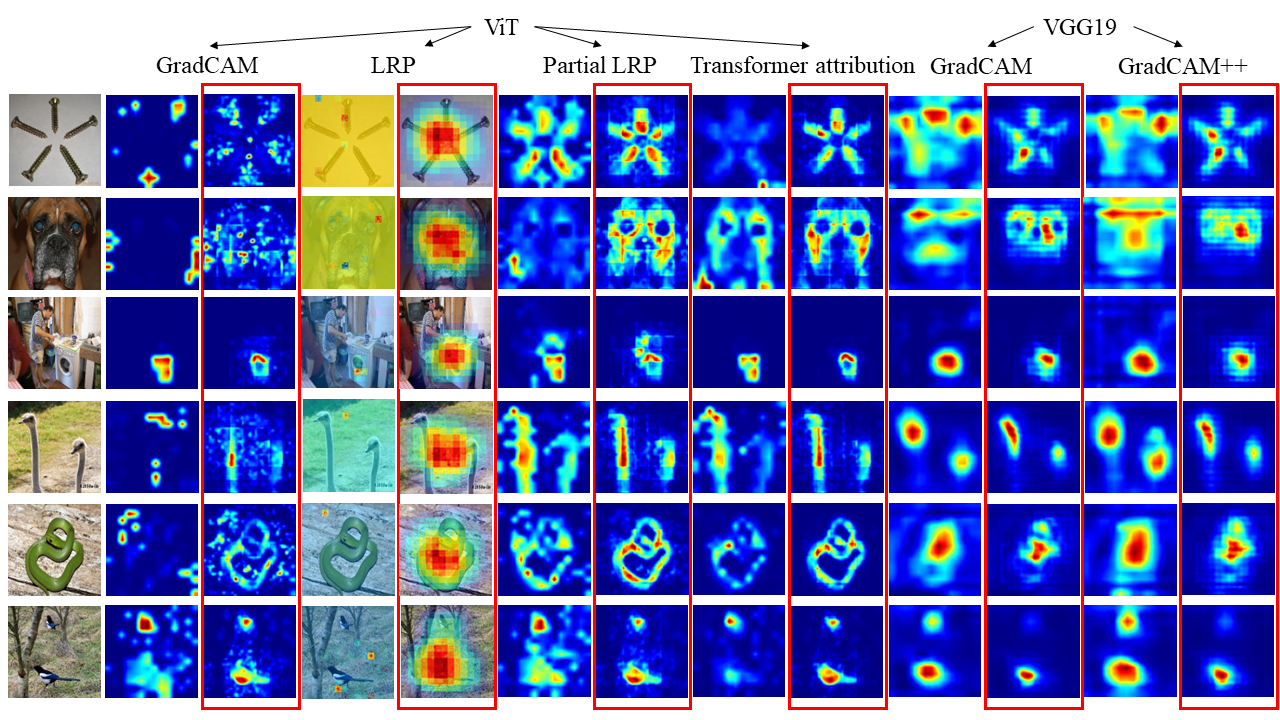
\includegraphics[width=15cm]{fig/ch4/Contrast.png}
	\bicaption[\xiaosi 增强方法应用于多种显著图解释方法上的直观对比结果]{\wuhao 增强方法应用于多种显著图解释方法上的直观对比结果}{\wuhao Intuitive comparison of enhancement methods applied to multiple saliency methods}
	%	\bicaption[\xiaosi MSG-CAM算法流程示意图]{\wuhao MSG-CAM算法流程示意图}{\wuhao Pipeline of MSG-CAM}
	\label{fig:contrast1}
\end{figure}

\begin{figure}[h]
	\centering 
	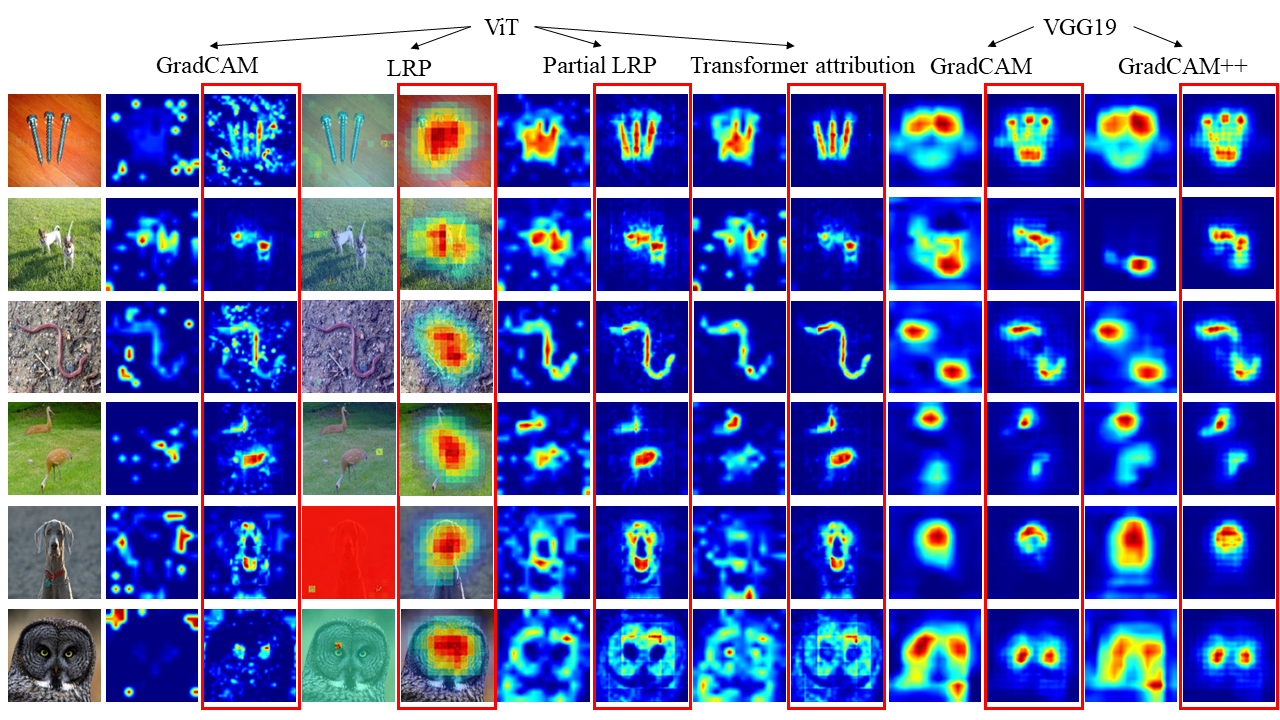
\includegraphics[width=15cm]{fig/ch4/Contrast1.png}
	\bicaption[\xiaosi 增强方法应用于多种显著图解释方法上的直观对比结果]{\wuhao 增强方法应用于多种显著图解释方法上的直观对比结果}{\wuhao Intuitive comparison of enhancement methods applied to multiple saliency methods}
	%	\bicaption[\xiaosi MSG-CAM算法流程示意图]{\wuhao MSG-CAM算法流程示意图}{\wuhao Pipeline of MSG-CAM}
	\label{fig:contrast2}
\end{figure}

\begin{figure}[h]
	\centering 
	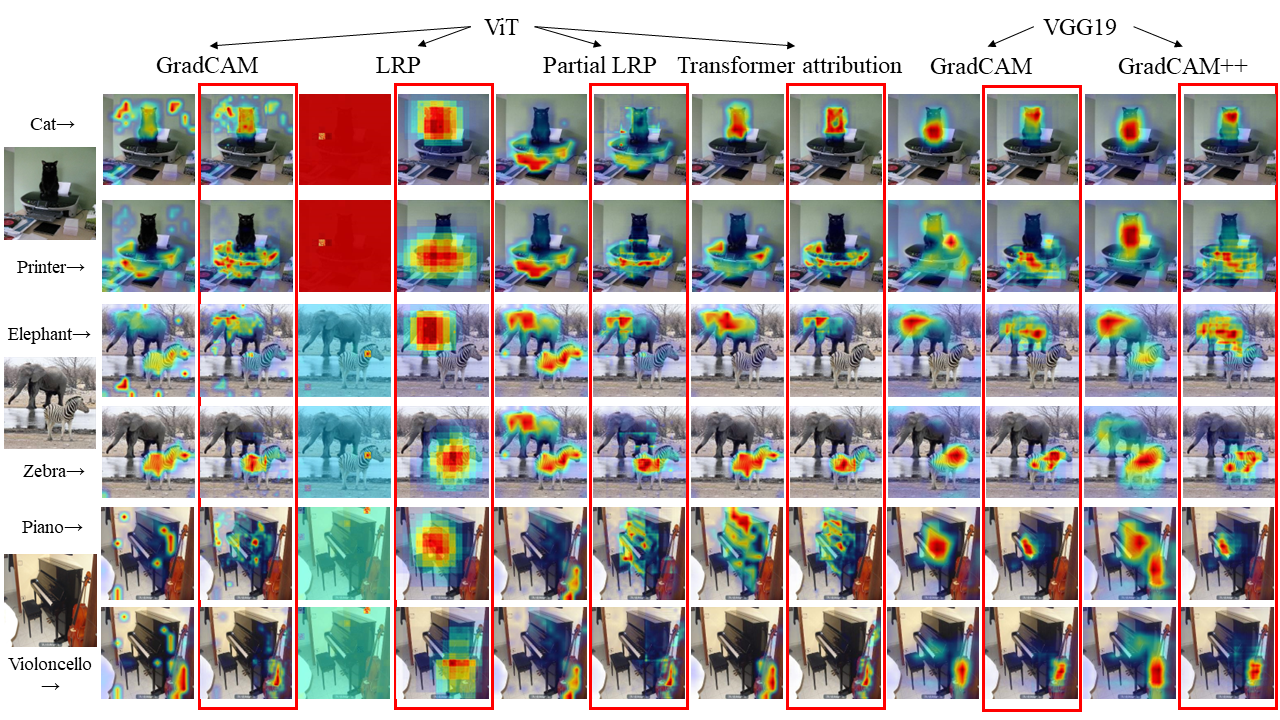
\includegraphics[width=15cm]{fig/ch4/classSensitive.png}
	\bicaption[\xiaosi 增强方法应用于多种显著图解释方法上的类别区分对比]{\wuhao 增强方法应用于多种显著图解释方法上的类别区分对比}{\wuhao Visual comparison of class distinctions of enhancement methods}
	%	\bicaption[\xiaosi MSG-CAM算法流程示意图]{\wuhao MSG-CAM算法流程示意图}{\wuhao Pipeline of MSG-CAM}
	\label{fig:classSensitive}
\end{figure}
\begin{table}
	\centering
	\renewcommand{\arraystretch}{1.5}
	\bicaption[\xiaosi 正负扰动实验数据对比]{\wuhao 正负扰动实验数据对比}{\wuhao Comparison of positive and negative perturbation experimental data}
	\wuhao
	\refstepcounter{table}
	\label{tab:pertubation}
	\resizebox{\linewidth}{!}{
		\begin{tabular}{ccccccccc} 
			\hline
			\multirow{2}{*}{模型}    & \multirow{2}{*}{显著图解释方法}                 & \multirow{2}{*}{增强算法} & \multicolumn{3}{c}{Predicted}                    & \multicolumn{3}{c}{Target}                        \\ 
			\cline{4-9}
			&                                          &                       & 负扰动            & 正扰动            & 总体             & 负扰动            & 正扰动            & 总体              \\ 
			\hline
			\multirow{8}{*}{ViT}   & \multirow{2}{*}{GradCAM}                 &                       & 41.52          & 34.06          & 7.46           & 42.02          & 33.56          & 8.46            \\ 
			\cline{4-9}
			&                                          & \checkmark                     & \textbf{47.54} & \textbf{26.99} & \textbf{20.55} & \textbf{48.46} & \textbf{26.49} & \textbf{21.97}  \\ 
			\cline{2-9}
			& \multirow{2}{*}{LRP}                     &                       & 43.49          & 41.94          & 1.55           & 43.49          & 41.94          & 1.56            \\ 
			\cline{4-9}
			&                                          & \checkmark                     & \textbf{62.69} & \textbf{27.51} & \textbf{35.18} & \textbf{64.76} & \textbf{26.45} & \textbf{38.31}  \\ 
			\cline{2-9}
			& \multirow{2}{*}{partial LRP}             &                       & 50.49          & 19.64          & 30.85          & 50.49          & 19.64          & 30.85           \\ 
			\cline{4-9}
			&                                          & \checkmark                     & \textbf{55.57} & \textbf{18.45} & \textbf{37.12} & \textbf{56.13} & \textbf{18.14} & \textbf{37.99}  \\ 
			\cline{2-9}
			& \multirow{2}{*}{Transformer attribution} &                       & 54.14          & 17.03          & 37.11          & 55.04          & \textbf{16.04} & 39.00           \\ 
			\cline{4-9}
			&                                          & \checkmark                     & \textbf{57.57} & \textbf{16.93} & \textbf{40.64} & \textbf{58.83} & 16.25          & \textbf{42.58}  \\ 
			\hline
			\multirow{4}{*}{VGG19} & \multirow{2}{*}{GradCAM}                 &                       & 38.08          & 12.15          & 25.93          & 39.04          & 11.71          & 27.33           \\ 
			\cline{4-9}
			&                                          & \checkmark                     & \textbf{39.07} & \textbf{10.20} & \textbf{28.87} & \textbf{40.09} & \textbf{9.78}  & \textbf{30.31}  \\ 
			\cline{2-9}
			& \multirow{2}{*}{GradCAM++}               &                       & 40.50          & 11.79          & 28.71          & 40.81          & 11.61          & 29.20           \\ 
			\cline{4-9}
			&                                          & \checkmark                     & \textbf{40.95} & \textbf{10.09} & \textbf{30.86} & \textbf{41.49} & \textbf{9.81}  & \textbf{31.68}  \\
			\hline
		\end{tabular}
	}
\end{table}
\subsection{扰动实验}
优秀的显著图解释算法要能准确找到神经网络做出决策的关键特征,并且在生成的显著图中对每个像素赋予它与其对决策贡献相匹配的数值。扰动实验就是在这一标准上比较不同显著图解释算法的性能。本章分别进行正负扰动实验,正负实验测试采用两阶段设置。首先,使用预先训练好的网络提取 ImageNet验证集的可视化图像。其次,逐渐屏蔽掉输入图像的像素,并测量网络的平均top-1准确率。在正扰动实验中,像素从相关度最高的像素被屏蔽到最低的像素,而在负扰动中,像素从最低的像素被屏蔽到最高的像素。在正向扰动中,可以看到性能急剧下降,这表明被遮挡的像素对分类得分很重要。在负扰动实验情况下,一个好的解释可以保持模型的准确性,同时去除与类别无关的像素。在这两种情况下,实验过程都测量计算了去除10\%-90\%像素时的曲线下面积(AUC)。这两项实验都可应用于图像分类模型预测结果类(Predicted)和真实标注类(Target)。在后一种情况下,特定类别的方法有望获得更好的性能,而与类别无关的方法则会在两种测试中表现出相似的性能。

正负扰动实验和插入删除实验本质是一致的,都是根据显著图给出的像素权值将输入图片中的像素删除来记录得到相关类别索引的概率分数的变化。在正负扰动实验当中,也可以用AUC(总体)来综合评价扰动实验结果,它的计算方式是AUC(总体)=AUC(负扰动)-AUC(正扰动)。从表1中可以看出,本章的增强算法在总体指标上都取得明显提升,其中提升最为显著的是ViT模型的可视化算法GradCAM和LRP,这是因为他们对ViT的可视化能力很差,无法定位关键特征,经过本章的方法增强后,初步具有定位关键特征的能力。这表明本章的方法可以帮助这些可视化算法找到神经网络感兴趣的关键特征,这在不同的模型上都是成立的。

从表\ref{tab:pertubation}中可以看出,本章的增强方法显著提高了所有"总体"得分。应用于ViT的Grad-CAM 算法和LRP算法的改进最为明显,这两种算法以前缺乏准确可视化和定位重要特征的能力。使用增强方法后,这些方法能够识别重要特征。图\ref{fig:contrast1}就是一个例子,它表明无论底层网络结构如何,本章的方法都能帮助显著性方法识别神经网络感兴趣的重要特征。






\begin{table}
	\renewcommand{\arraystretch}{1.5}
	\centering
	\bicaption[\xiaosi 显著图增强算法在图像分割的表现]{\wuhao 不同的显著图解释方法应用增强算法前后图像分割的表现}{\wuhao Performance of saliency map enhancement algorithms for image segmentation}
	\wuhao
	\label{tab:seg}
	\resizebox{\linewidth}{!}{
		\begin{tabular}{cccccc} 
			\hline
			模型                     & 显著图解释方法                                  & 增强算法 & Pixel Acc(\%)      & mAP(\%)             & mIoU(\%)             \\ 
			\hline
			\multirow{8}{*}{ViT}   & \multirow{2}{*}{GradCAM}                 &      & 64.44          & 71.60          & 40.82           \\ 
			\cline{3-6}
			&                                          & \checkmark    & \textbf{70.33} & \textbf{77.02} & \textbf{47.81}  \\ 
			\cline{2-6}
			& \multirow{2}{*}{LRP}                     &      & 51.09          & 55.68          & 32.89           \\ 
			\cline{3-6}
			&                                          & \checkmark    & \textbf{69.34} & \textbf{80.88} & \textbf{50.37}  \\ 
			\cline{2-6}
			& \multirow{2}{*}{partial LRP}             &      & 76.31          & 84.67          & 57.94           \\ 
			\cline{3-6}
			&                                          & \checkmark    & \textbf{80.42} & \textbf{85.83} & \textbf{62.85}  \\ 
			\cline{2-6}
			& \multirow{2}{*}{Transformer attribution} &      & 79.74          & 86.03          & 62.01           \\ 
			\cline{3-6}
			&                                          & \checkmark    & \textbf{81.90} & \textbf{86.56} & \textbf{64.56}  \\ 
			\hline
			\multirow{4}{*}{VGG19} & \multirow{2}{*}{GradCAM}                 &      & 69.03          & 76.76          & 48.99           \\ 
			\cline{3-6}
			&                                          & \checkmark    & \textbf{73.78} & \textbf{79.99} & \textbf{53.82}  \\ 
			\cline{2-6}
			& \multirow{2}{*}{GradCAM++}               &      & 76.77          & \textbf{85.48} & 58.89           \\ 
			\cline{3-6}
			&                                          & \checkmark    & \textbf{78.60} & 85.42          & \textbf{60.58}  \\
			\hline
		\end{tabular}
	}
\end{table}


\subsection{图像分割实验}
图像分割实验将每张显著图视为图像的软分割,并将其与ImageNet-Segmentation数据集的真实标注的分割进行比较。在分割实验中,计算每个突出图中像素的平均值,并将突出图中高于平均值的像素设为 1,其余像素设为 0。本节使用语义分割中常用的三个指标来衡量性能:像素精确度(Pixel Accuracy)、平均交叉重叠率(mIoU)和平均精确度(mAP),其中mIoU即对每张显著图进行平均值阈值化处理后获得的准确度,mAP是使用不含阈值的显著图计算得出的。

分割结果如表\ref{tab:seg}所示。从中可以看出,本章的增强方法在所列的像素精确度(Pixel Accuracy)、平均交叉重叠率(mIoU)和平均精确度(mAP)关键指标,上都有显著的改进,甚至 Transformer attribution\textsuperscript{\cite{chefer2021transformer}} 也能获得不可忽略的改进,这是目前在基于Transformer架构上的图像分类神经网络ViT模型上表现最好的方法。这表明,本章的增强方法可以帮助提高当前显著图解释方法在分割领域的性能。

	
\section{本章小结}
本章首先分析当前显著图生成方法普遍存在的低分辨率问题的原因,然后本章详细介绍了一种通用的基于二维滑动窗口和放大的图像分类神经网络显著图解释增强方法,该方法无须改变当前既有的显著图生成方法的内部计算流程,只需要关注输入的原始图片和输出的概率分数即可完成对当前既有显著图生成方法的增强。增强后的显著图具有更高的分辨率和更精准的特征定位。为了使得因滑动窗口导致的显著图不够平滑的问题,本章的方法还使用了低通滤波器对其平滑。最后本章设计了扰动实验,选取了多个显著图生成方法和两个不同架构的图像分类网络来验证本章增强方法的有效性,经过直观对比和数据对比,本章的显著图增强方法都取得了明显效果。 

